\newcommand{\COMMENT}[1]{\noindent\fbox{\parbox{0.98\linewidth}{\bfseries #1}}}


\chapter{Fundamentação Teórica}
\label{ch:fundamentos}

Este capítulo introduz os conceitos necessários para a compreensão do restante do trabalho. A Seção~\ref{sec:introDNS} apresenta o \textit{Domain Name System} (DNS). A Seção~\ref{sec:introHoney} discute \textit{honeypots}. Na seção~\ref{sec:introDNSpot} é descrito o DNSpot, um \textit{honeypot} específico para servidores DNS recursivos.

\section{Domain Name System}
\label{sec:introDNS}

O \textit{Domain Name System} (DNS) desempenha uma funcionalidade essencial para a operação da Internet, sendo responsável por, entre outras funcionalidades, realizar a associação de um nome de domínio com um endereço IP. O sistema é implementado como uma estrutura hierárquica, possuindo servidores raiz, que são responsáveis por atualizar a lista de nomes e endereços IPs \cite{Gao:2013}.


\subsection{Definição}
\label{sec:defiDNS}

DNS é um sistema distribuído de banco de dados, cujo objetivo original
era permitir que recursos de rede sejam identificados por nomes em vez
de endereços de baixo nível \cite{rfc1034}. Em particular, o DNS
permite que usuários refiram-se a nós da rede usando nomes (como
\url{www.udesc.br}) no lugar dos endereços IP (como 200.19.105.51)
efetivamente usados para a comunicação entre esses nós. Ao longo do
tempo, o escopo do DNS foi ampliado, basicamente devido a sua ampla
disseminação, passando a associar vários tipos diferentes de dados a
nomes de domínio \cite{rfc3467}. Dada a sua estrutura com abrangência
global e a sua ubiquidade, o DNS deve ter boa escalabilidade e
desempenho, oferecendo para os usuários baixa latência em redes de
larga escala \cite{Jung:2002}. O DNS é crítico para o funcionamento da
maioria dos serviços encontrados na Internet: embora sempre seja
possível referir-se a um nó (por exemplo, um servidor web) usando seu
endereço IP, os usuários buscam resolver os endereços utilizando o seu
nome \cite{dnsmonitoring}. Além disso, o DNS introduz uma camada de
indireção, permitindo, por exemplo, que um nó mude seu endereço IP de
forma transparente para os usuários e aplicações que desejem se
comunicar com ele.


% O DNS é um sistema simples que permite uma \textit{string}, juntamente com um domínio de serem consultadas em \textit{database}, retornando uma resposta para o usuário, ou uma resposta que o endereço não existe \cite{Conrad:2012:tidssr}.


\subsection{Hierarquia}

O espaço de nomes do DNS segue uma estrutura em árvore
\cite{rfc1034}. A cada nó da árvore, seja um nó interno ou uma folha,
corresponde um conjunto de recursos, que pode ser vazio. Cada nó possui
um rótulo com até 63 bytes de comprimento. Nós irmãos devem ter
rótulos distintos, mas o mesmo rótulo pode ser usado para nós que não
são irmãos. A raiz da árvore possui um rótulo com comprimento zero,
tipicamente representado por um ponto (``.''). O nome de domínio de um
nó é a lista de rótulos que formam o caminho do nó até a raiz da
árvore. Por exemplo, na árvore DNS mostrada na Figura, o nó mais à
esquerda possui o nome de domínio \url{irs.treasury.gov.}; em geral, o
ponto final é omitido, quando isso não causar ambiguidade.

\COMMENT{%
    \begin{enumerate}
    \item eliminar a parte de UNIX da figura
    \item incluir um rótulo ``irs'' em outra subárvore, e mostrar que eles podem coexistir
\end{enumerate}}

    \begin{figure}[ht]
        \centering
        \includegraphics[width=0.9\textwidth]{pictures/tree.png}
        \caption{DNS vs UNIX estrutura}
        \label{fig:tree}
    \end{figure}

Na árvore DNS, cada subárvore é um domínio. Um conceito chave no DNS é a administração descentralizada, que consiste em delegar a administração de domínios a entidades autônomas \cite{Mockapetris:1988}. A administração de um domínio engloba a criação de nós nesse domínio e a definição dos recursos associados a nomes pertencentes ao domínio. Cada domínio possui um ou mais servidores responsáveis pelos seus nomes,  chamados de servidores autoritativos. Em geral, esses servidores são configurados de forma que um deles (servidor primário ou mestre) é o repositório central de dados para o domínio, e os demais (servidores secundários ou escravos) apenas replicam  os dados do servidor primário para oferecer balanceamento de carga e tolerância a falhas \cite{Liu:2006}. A divisão entre servidores mestres e escravos é transparente para os usuários do DNS\@.

\COMMENT{Reaproveitei a citação, mas a ordem correta dos autores é (Albitz e Liu 2006), não (Liu e Albitz 2006).}

A figura \ref{fig:delegation} ilustra a delegação do subdomínio
\url{treasury.gov} pelo domínio \url{gov}. A delegação é efetivada
atribuindo-se um conjunto de servidores autoritativos que irão
administrar os nomes em \url{treasury.gov} de forma autônoma. Um
conceito associado ao de domínio é o conceito de zona, que abrange
todas as partes de uma subárvore que não estão delegadas; por exemplo,
na figura~\ref{fig:delegation} a zona \textit{gov} contém nomes de
domínios que forem terminados em \textit{gov} e não estejam em nenhuma
zona de delegação.

\COMMENT{%
    \begin{itemize}
    \item Parece-me que seria mais fácil visualizar a delegação de um subdomínio de 3o nível (por exemplo, \url{cct.udesc.br}; a zona \url{udesc.br} conteria \url{ceart.udesc.br} mas não \url{cct.udesc.br}). A delegação de um domínio de 2o nível (como \url{treasury.gov}), embora tecnicamente seja a mesma coisa, é mais difícil de visualizar, pois as pessoas têm dificuldade de imaginar um domínio \url{gov}.
    \item Também neste caso retire a árvore de UNIX
\end{itemize}
}

    \begin{figure}[ht]
        \centering
        \includegraphics[width=0.9\textwidth]{pictures/Delegating.png}
        \caption{DNS vs UNIX Delegação }        
        \label{fig:delegation}
    \end{figure}
    \FloatBarrier

% A hierarquia do DNS consiste de uma árvore, onde na raiz da árvore está contido o domínio, e os filhos deste domínio estariam localizados no primeiro nível, cada um podendo conter diversos subdomínios. As informações de cada domínio são armazenadas em um servidor autoritativo, através deste servidor existe a necessidade de pesquisar em outras estruturas, possuindo o compartilhamento de informação para realizar a busca dos dados \cite{Liu:2006}.

% A figura \ref{fig:tree} demonstra um comparativo entra a estrutura do DNS com o sistema de arquivos do UNIX. Toda estrutura é representa por uma árvore invertida, na qual a aresta \textit{`` " ou /} (representando o \textit{root}), é encontrada no topo da árvore invertida. Cada aresta possui um rótulo, que contem as relações da aresta.

%     \begin{figure}[ht]
%         \centering
%         \includegraphics[width=0.9\textwidth]{pictures/tree.png}
%         \caption{DNS vs UNIX estrutura }        
%         \label{fig:tree}
%     \end{figure}
%     \FloatBarrier

% Cada aresta vai ser um \textit{root} de uma nova subárvore, representando uma partição da estrutura, tanto para a estrutura do DNS como para o UNIX. Um subdomínio é uma divisão que pode ser apresentada no domínio (DNS) ou diretório (UNIX), que representa um nova partição ao domínio. O nome do domínio vai demonstrar sua posição no \textit{database}, como também seria observado no UNIX através do nome do diretório. O domínio vai representar a sequência de rótulos, iniciando na raiz (\textit{root}), separado por pontos (.) \cite{Liu:2006}.

% A realização de uma busca na figura \ref{fig:tree}, vai possuir algumas diferenças entre as duas estruturas. No caso a busca no DNS vai seguir o caminho contrário em relação a busca no UNIX, como segue:

% $\implies irs \implies treasury \implies gov$

% \textit{irs.treasury.gov}

% $\implies / \implies usr \implies local \implies bin \implies imake$

% \textit{/usr/local/bin/imake}

% Pode existir a criação de uma nova zona administrada de forma autônoma, que seja independente da outra, contendo todos os nomes de domínio necessários. Na figura \ref{fig:delegation} é possível observar a criação de uma nova zona \textit{irs.treasury.gov} onde \textit{irs.treasury} agora é independente da \textit{gov}, possuindo todos os domínios necessários. A zona \textit{gov} só contém nomes de domínios que forem terminadas em \textit{gov} e não estejam em nenhuma zona de delegação.

%     \begin{figure}[ht]
%         \centering
%         \includegraphics[width=0.9\textwidth]{pictures/Delegating.png}
%         \caption{DNS vs UNIX Delegação }        
%         \label{fig:delegation}
%     \end{figure}
%     \FloatBarrier
    
A solução de um domínio como \textit{host.tex}

%%%Terminar com a solução de um dominio host.tex

\subsection{Resolução de nomes}


%%%explicar a resolução de nome (definição no livro)

\subsection{Fatores de Segurança}

%%%Artigo/Livro

\subsection{Nome de Domínio}

%%%Só comentar

\section{Honeypot}
\label{sec:introHoney}

\COMMENT{A mensagem aqui deveria ser que honeypots oferecem uma forma controlada de observar o comportamento dos atacantes, o que é importante para conhecer suas táticas, motivações e ferramentas e assim poder criar novas defesas ou melhorar as defesas existentes. Pontualmente, a última frase é aproveitável, mas as duas primeiras precisam ser reescritas.}

Ataques são realizados após uma massiva busca por falhas de seguranças, ao encontrarem falhas existe a tentativa de invasão de uma determinada rede.
Uma maneira desenvolvida para a identificação, análise ou controle destas tentativas de invasão é o \textit{honeypot}. Sua mentalidade é a de criar um ambiente isolado onde se possa monitorar tentativas de ataques em uma determinar rede, visando armazenar informações dos ataques recebidos.

   
    
\subsection{Definição}
\label{sec:defiHoney}

\COMMENT{Inclua uma referência ao final da 1a frase.}

O \textit{honeypot} é um recurso computacional com o objetivo de ser sondado, atacado ou até mesmo comprometido. Geralmente o \textit{honeypot} é um \textit{host} Internet, possuindo um endereço IP público, mas que não hospeda nenhum serviço anunciado publicamente. Qualquer interação realizada com o \textit{honeypot} já pode-se considerar suspeita, já que é necessário a realização de uma varredura para a descoberta do endereço de IP do \textit{honeypot}. O sistema deve ser monitorado de forma discreta, para garantia que o atacante não suspeite do sistema, e acabe descobrindo o seu monitoramento \cite{honey:2007}. %%%%%%%%%%%CITE CERT HONEYPOT PAGE

A estrutura que pode ser observada na figura \ref{fig:honey}, leva em consideração o funcionamento do \textit{honeypot} em uma rede, como retratado buscando esconder quaisquer suspeitas que um usuário que busque atacar a rede consiga identificar.

\COMMENT{%
  \begin{itemize}
  \item Em relação à figura, é muito pouco recomendável colocar o
    honeypot junto da rede interna, o melhor seria colocá-lo como uma
    perna adicional do firewall. Observo aqui que o DNSpot está na
    nossa rede interna, mas isso só ocorre porque ele é um honeypot
    para uma aplicação específica, e a conveniência de mantê-lo na
    rede interna compensa o pequeno risco de que ele seja comprometido
    e usado como plataforma para outros ataques.
  \item Outro ponto é que olhando a figura o leitor não consegue ver nenhum elemento que permita que o honeypot não desperte suspeitas. Esse ponto, aliás, já é tratado na última frase do parágrafo anterior, e pode ser omitido aqui. Sugiro colocar uma figura e explicar de que forma colocar o honeypot em uma rede segregada, por exemplo, facilita a monitoração e a contenção do tráfego; se quiser, acrescente a necessidade de contenção de tráfego originado no honeypot no parágrafo anterior.
  \end{itemize}
}


    \begin{figure}[ht]
        \centering
        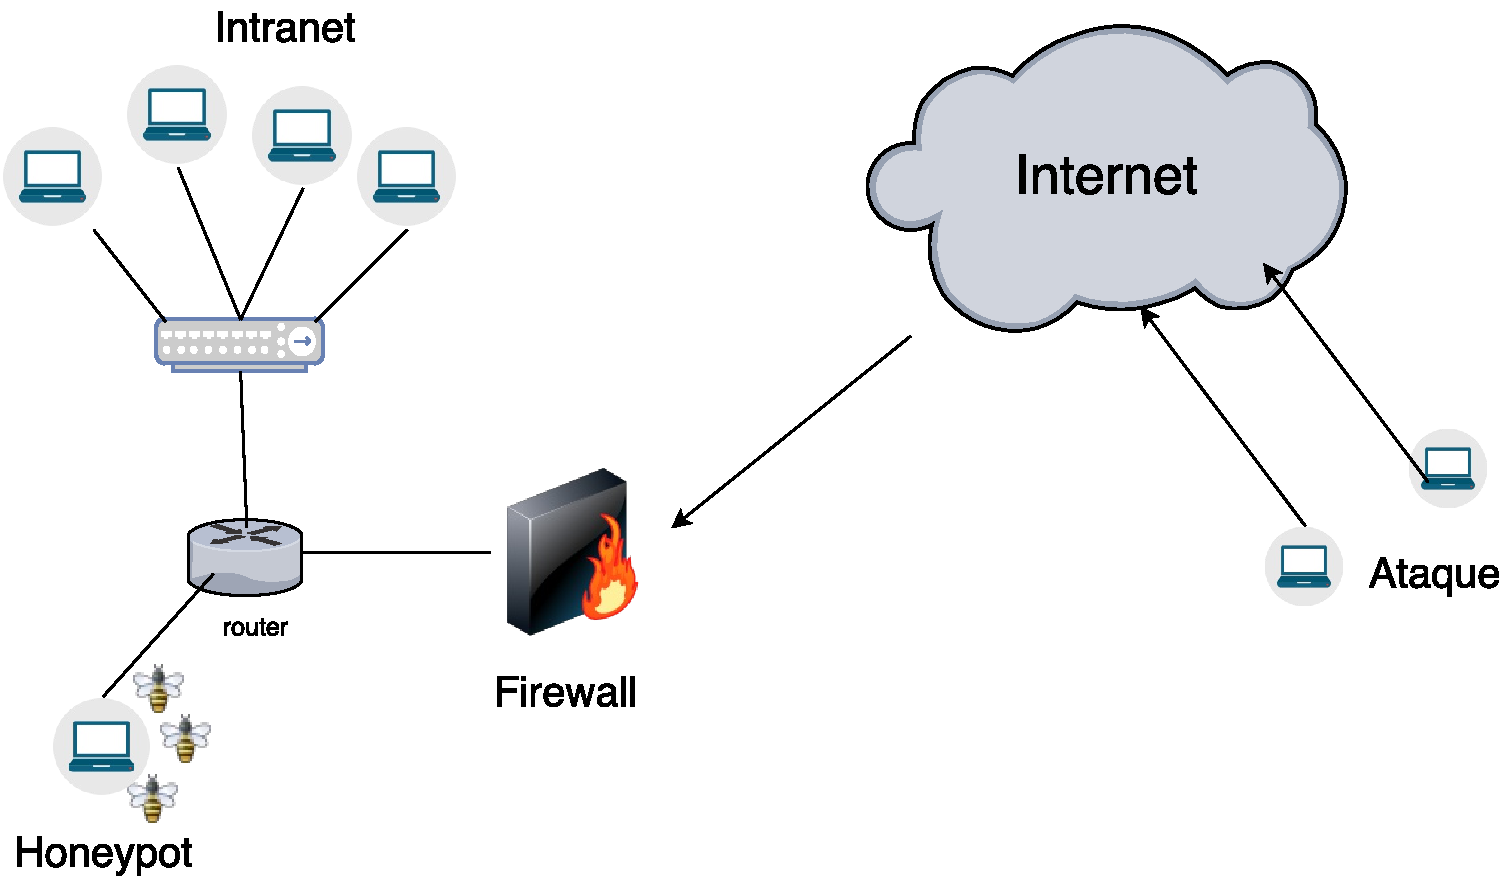
\includegraphics[width=0.9\textwidth]{pictures/honeypot.pdf}
        \caption{Honeypot}        
        \label{fig:honey}

    \end{figure}
    \FloatBarrier

\subsection{Honeynet}
\label{sec:honey1}

\COMMENT{Cuidado, uma honeynet é uma rede que abriga um conjunto de honeypots, geralmente distintos (por exemplo, usando sistemas operacionais diferentes). Essa discussão que você colocou aqui sobre a estrutura da rede pode aplicar-se quase da mesma forma a um honeypot isolado, pois ele precisa de elementos auxiliares para prover conectividade, monitorar e conter o tráfego.}

Uma \textit{Honeynet} é considera uma rede onde o \textit{Honeypot} está localizado, retratando os dispositivos que compõem esta estrutura. Uma \textit{Honeynet} pode estar composta por alguns elementos como: 

	\begin{itemize}
		\item A estrutura pode ser composta por diversos computadores;
		\item \textit{Firewall}, responsável pela realização de contenção e coleta de informações;
		\item IDS (Intrusion Detection System) tem o objetivo de observar a rede, buscando atividades em comum ou não autorizadas que podem danificar o sistema;
		\item roteadores, \textit{switches} e hubs para a composição da estrutura de rede \cite{honey:2007}%cite\ link
%http://www.cert.br/docs/whitepapers/honeypots-honeynets/
	\end{itemize}

O baixo custo e a interação do atacante com um ambiente real, contribuem com um estudo sobre as ferramentas utilizadas e vulnerabilidades exploradas.

\COMMENT{O parágrafo abaixo confunde conceitos. Uma honeynet virtual consiste em um conjunto de honeypots implementados em máquinas virtuais em um mesmo host físico (cf. \url{http://old.honeynet.org/papers/virtual/}); em uma honeynet real, cada honeypot é um host físico separado. Um honeypot/honeynet de pesquisa tem o propósito de estudar o comportamento dos atacantes; em contrapartida, um honeypot/honeynet de produção tem o objetivo de detectar ataques e responder a eles (cf. \url{http://www.it-docs.net/ddata/792.pdf}, p. 62). Acho que uma ideia aqui é pensar o que você \textbf{precisa} explicar para tornar o texto autocontido. Não vejo muito sentido em esmiuçar conceitos de honeypots e honeynets porque você não vai propor uma nova ferramenta, mas usar uma que já existe; o importante é que o leitor entenda o que é o DNSpot e suas principais características, e não que ele raciocine sobre as escolhas de projeto do DNSpot (isso compete ao TCC do Felipe).}

Existem duas classificações para os \textit{honeypots}, uma rede projetada especificamente para ser atacada e testada, visando a utilização de mecanismo de controle é conhecida como \textit{honeynet}, e uma rede com alta interatividade que busca obter informações dos usuários que estão realizando o ataque, também conhecida como \textit{honeynets virtuais} ou \textit{honeypot} de pesquisa \cite{honey:2007}.

\subsection{Aplicação}

Os \textit{honeypots} podem ser classificados em duas categorias, \textit{honeypot} de alta e baixa interatividade (como apresentado na \ref{sec:honey1}). O \textit{honeypot} de baixa interatividade busca identificar ataques internos e varreduras, também realiza identificação de máquinas comprometidas e códigos maliciosos. Já por outro lado o \textit{honeypot} de alta interatividade apresenta risco para a rede, podendo ser utilizado com o mesmo propósito do \textit{honeypot}  de baixa interatividade, seu principal objetivo é estudar o comportamento  detalhadamente dos atacantes, juntamente com técnicas e ferramentas utilizadas para explorar alguma vulnerabilidade \cite{honey:2007}.

 

\subsubsection{Aplicação na rede}    

%%%Utilização do honeynet

\section{DNSpot}
\label{sec:introDNSpot}

O DNSpot é um \textit{honeypot} projetado especificamente para monitorar e analisar o tráfego DNS \cite{Longo:2015:tcc}. Seu objetivo é permitir a observação das interações de usuários potencialmente maliciosos com servidores DNS recursivos. %%%felipe


\subsection{Definição}
\label{sec:defiDNSpot}

%%%%%%%FUNCIONAMENTO

\subsection{Arquitetura}
A arquitetura do DNSpot pode ser observada na figura \ref{fig:dnspot}. Ele possui um \textit{proxy} que escuta na porta 53/UDP, que é a porta padrão do serviço DNS\@. Ao receber uma consulta, o \textit{proxy} será responsável por armazenar a consulta em um banco de dados e logo em seguida repassá-la a um servidor DNS recursivo real. Esse servidor real, que aceita apenas consultas originadas na própria máquina, vai interagir com servidores autoritativos na Internet para a resolução desta consulta. Por último, o \textit{proxy} irá receber a resposta do servidor recursivo, armazená-la no banco de dados e encaminhá-la para o cliente que enviou a consulta \cite{Longo:2015:tcc}.


    \begin{figure}[ht]
        \centering
        \includegraphics[width=0.9\textwidth]{pictures/dnspot.png}
        \caption{Arquitetura DNSpot}        
        \label{fig:dnspot}

    \end{figure}
    \FloatBarrier


\COMMENT{O texto abaixo confunde dois mecanismos distintos. O SERVFAIL aleatório é para simular um servidor DNS inconfiável, tentando não levantar suspeitas caso o DNSpot seja desligado ou não consiga processar algumas consultas. Por sua vez, a limitação de consultas funciona como um mecanismo de contenção do tráfego gerado pelo DNSpot; ele permite que um usuário humano interaja com o honeypot, mas restringe a quantidade de tráfego gerada em caso de ataques de DoS por reflexão.}

O critérios de decisão escolhidos foram dois:

\begin{enumerate}

	\item Randomização: uma porcentagem é definida para as consultas, determinando se receberão uma resposta em tempo real ou não, e o \textit{proxy} faz uma decisão aleatória para determinar se será respondido a consulta ou será retornado um erro;

	\item Limitação: um limite diário é determinado para o número de consultas atendidas para cada endereço IP de origem; caso o limite seja atingido o \textit{proxy} passa a ignorar novas consultas do mesmo endereço,  até o dia seguinte (onde a atividade é retornada novamente) \cite{Longo:2015:tcc}.
	
\end{enumerate}

\section{Estatísticas}
\label{sec:introEsta}

\COMMENT{Acho que aqui você queria comentar os resultados do DNSpot, certo? Nesse caso, deveria ser uma \textit{subsection}, não uma \textit{section}.}

%%% Falar sobre a estatisticas e resultados 
%%%estatisticas DNSpot section